\chapter{Fűtőtestek modellje}\label{chap:futotest}

A fűtőtestek feladata, hogy az adott szobában teljesítményt szolgáltassanak, hőt\footnote{A hő mértékegysége \si{\joule}, a teljesítményé [\si{\watt}]~=~[\si[per-mode=fraction]{\joule\per\second}]} adjanak le. A fűtőtest teljesítményével növeli a környezet hőjét:
%, így a levegő és az épületszerkezetek felmelegszenek. 
a levegőnek konvektív hőátadás útján, légáramlással, a környezetnek pedig radiatív hőátadással, azaz hősugárzással.
%a levegő

Ebben a fejezetben először hőtani alapösszefüggéseket ismertetek, amelyekből előáll majd a fűtőtestek teljesítményét leíró modell. Az állandósult állapotban leadott hő megkapható a beavatkozó jelek és a környezeti jellemzők (mért hőmérsékletek) függvényében (\textit{\ref{eq_holeadas4}. egyenlet}).
A modell által számolt teljesítményt egy Simscape-ben megvalósított termikus hálózatra vezetem\footnote{A termikus hálózatok alkotóelemeiben a hővezetési tényezők és határoló elemek megfeleltethetők ellenállásoknak és kondenzátoroknak.}, ami a fűtőtest tranziens viselkedését adja meg. Az alábbi ábrán látható ezen rendszerek kapcsolata. 
%A fűtőtestek kimenetei a helyiség modelljének bemenetére csatlakoznak.

\begin{figure}[H]
	\centering
	% trim={<left> <lower> <right> <upper>}
	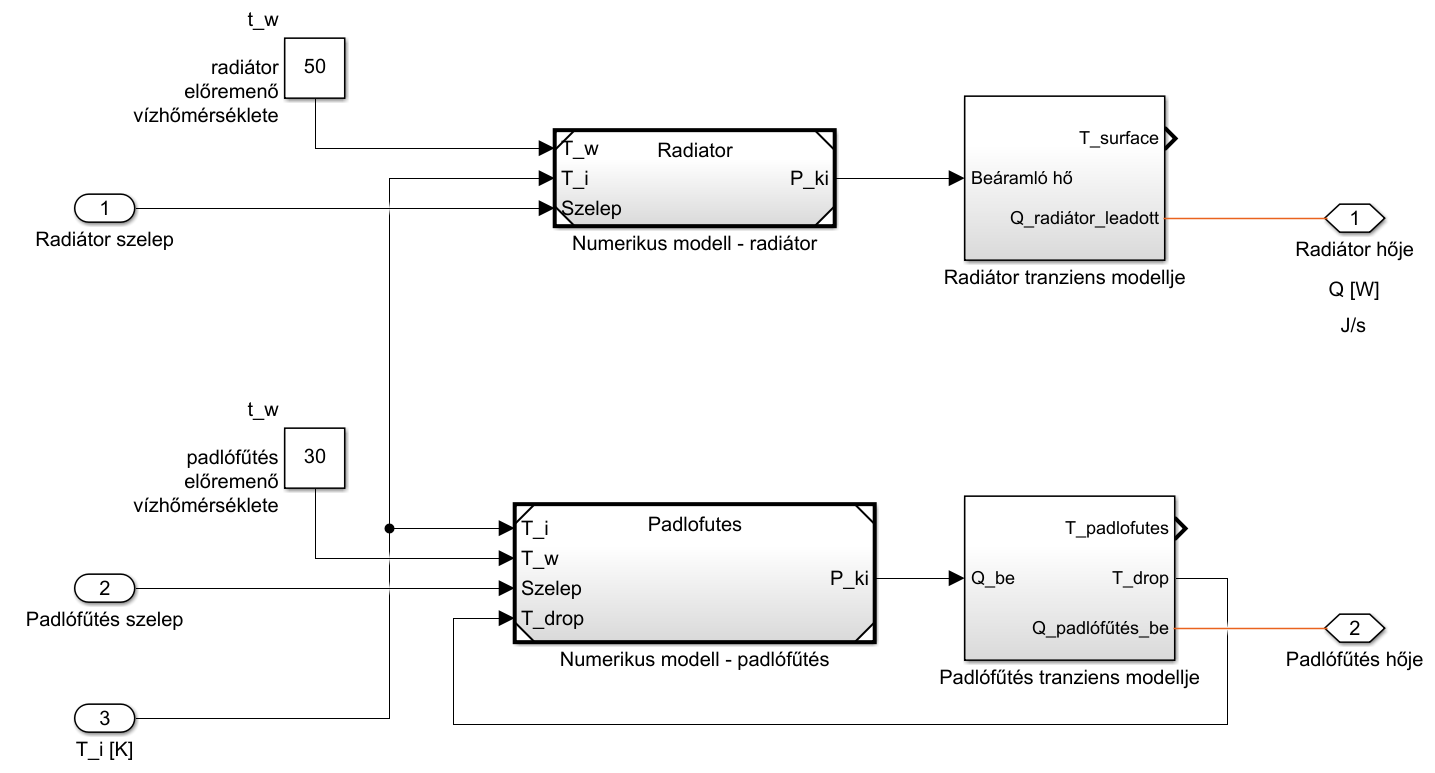
\includegraphics[trim=0 0 0 0, clip,width=0.9\textwidth]{figures/simscape/heatsys}
	\caption{Fűtőtestek modellje}
	\label{fig:SimscapeHeatSys}
\end{figure}



%Szimuláció során olyan bekapcsolási tranziensekkel is számolnom kell, amik egy kis időállandós fűtés (pl. légbefúvás, fan-coil) esetén elhanyagolhatók lennének.
%A modellalkotás során kétféle probléma merül fel. Egyrészt modellezni kell a fűtőtestek állandósult állapotbeli hőleadást. Másrészt, ha a fűtési rendszer időállandója nagy, akkor a tranziens lefolyása is lényeges a szabályzás szempontjából.
\section{Állandósult állapotbeli hőleadás numerikus modellje}\label{section:allandosult}

Mivel a vizsgált fűtési rendszerek hője melegvízből származik, a fűtővíz %kazán (hőszivattyú, stb.) által előállított melegvíz
hőmérséklete, illetve a keringető szivattyú tömegárama lehet a hőleadást befolyásoló paraméter\footnote{A kazánok a víz hőmérsékletét képesek változtatni időjárás függvényében, így az egy külön rendszer része lehet. Nem célom kazánvezérlést írni, az egyszerűség kedvéért feltételezem, hogy a melegvíz például távhő formában rendelkezésre áll.}. Az elképzelésemmel jobban összhangban áll az utóbbi választása, hiszen szelepekkel elosztottan, szobánként is szabályozható az egyes fűtőtestekbe táplált hőmennyiség: a víz tömegáramát folytonosan tudom szabályozni egy szelep segítségével\footnote{A \textit{\ref{chap:feasibility-tech}. részben} mutatom be a megvalósíthatóság technikai feltételeit, például azt, hogy milyen szelep használatos erre a feladatra.}, a fűtőtestekbe betáplált víz hőmérséklete (úgynevezett előremenő hőmérséklet) állandó.

%\vspace{6pt}

A fűtőtest hőleadása függ a környezetétől is. A szabályzott jellemzőn felül a modell bemenetéhez tartozik a környezet hőmérséklete, ami a levegő vagy a fűtetlen objektumok hőmérséklete\footnote{A hőleadás típusa dönti el, hogy ezek közül melyik mérvadó. Különböző típusú fűtőtesteknél a teljesítmény más-más arányban oszlik meg konvektív és radiatív hőátadás között.}.
Ezen bemenő paraméterek és a fizikai tulajdonságok alapján megadható az állandósult állapotbeli teljesítmény. Ennek levezetése ebben a bekezdésben található.

A tranziensek a fűtőtestek fizikai kialakításától függnek. Minél nagyobb tömeget kell átmelegíteni azelőtt, hogy a fűtőtest felszínén a hőleadás megindulna, annál lassabb a beállási ideje az állandósult állapotnak. Kikapcsoláskor a fűtőtest a szelep elzárása után is ad le hőt. %Így egy adott referencia trajektória esetén figyelembe kell venni ezen rendszerek dinamikáját is.
A hőtárolási paramétereket könyvekből, publikációkból, gyártói katalógusokból, méréssel, vagy becsléssel határoztam meg. A Simscape-ben minden blokknak olyan fizikai tartalma van, amiben ezek a jellemzők bevihetők, hatásuk megfigyelhető. Ezt a modellt a \textit{\ref{section:dinamikus}. bekezdésben} láthatjuk.
%A modellhez szükség van pl. a fűtőtest felületi hőmérsékletének, vagy a visszatérő (lehűlt) víz hőmérsékletének mérésére.% A modellezéshez korlátozottan áll rendelkezésre információ, ugyanis nem 

%\textbf{\textit{TIKZPICTURE A MODELLRŐL, DIMENZIÓKRÓL}}

%\begin{figure}[h]
	\centering
	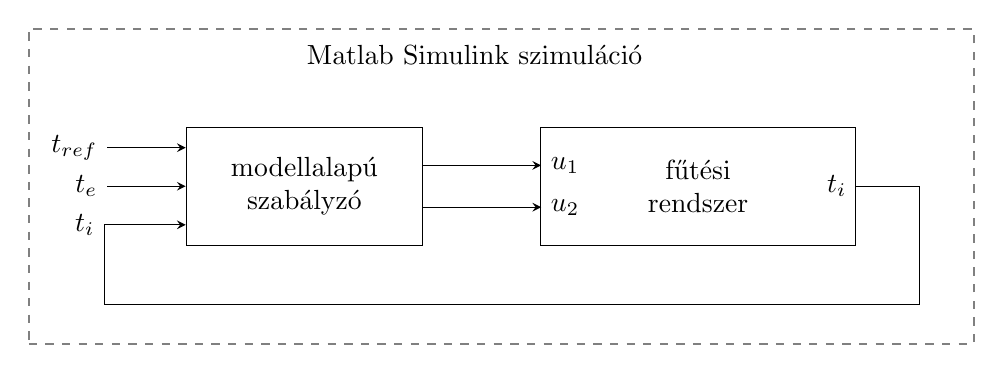
\begin{tikzpicture}[>=stealth,
	outer/.style={draw=gray,dashed,thick,inner sep=5pt}]

	% nagy blokkok
	\node[draw,rectangle, minimum height=1.5cm,minimum width=4cm] (plant) at (5,2.5) {\parbox{2cm}{\centering fűtési rendszer}};
	\node[draw,rectangle, minimum height=1.5cm,minimum width=3cm] (Control) at (0,2.5) {\parbox{2.5cm}{\centering modellalapú\\szabályzó}};
	
	% szaggatott vonal
	\node[draw,outer,rectangle, minimum height=4cm,minimum width=12cm,
	label={[label distance=-0.1cm, anchor=north]100:Matlab Simulink szimuláció}] (keret) at (2.5,2.5) {};
	
	
	% szabályzott mennyiségek
	\draw [->] (Control.10) node[right]{} -- +(15mm,0) node[right]{${u_{1}}$};
	\draw [->] (Control.350) node[right]{} -- +(15mm,0) node[right]{${u_{2}}$};
	
	%\draw[->] (Control.350) node[left]{} --  (plant.187) node[right]{${u_{2}}$};  %node[above left]{$\alpha_{radiator}$}; 
	%\draw[->] (Control.10) node[left]{} --  (plant.173) node[right]{${u_{1}}$} ;
	
	%\draw[->] (d.0) node[left]{heat [W]} ->  ++(3,0) ->  (house.180);
	
	
	% szabályzó bemenetei
	% a -| és |- máshogy fog törni, ha unconstraintelt.
	\draw [->] (plant.0)  node[left]{$t_i$} -|++(0.8,-1.5) -| ++(-9.25,0) |-  ++(-1.1,0) |- node[left]{$t_i$} (Control.198);
	
	%++(1.5cm,0) -- (2cm,0pt) -- (2.5cm,10pt);
	%\draw [->] (plant.0) node[left]{$t_i$ [\si{\celsius}]} -|++(1,0)|- -|++(-2.5,0)|- (Control.198) node[right]{}; %++(1.5cm,0) -- (2cm,0pt) -- (2.5cm,10pt);
	\draw [<-] (Control.180) node[right]{} -- +(-10mm,0) node[left]{$t_{e}$};
	\draw [<-] (Control.162) node[right]{} -- +(-10mm,0) node[left]{$t_{ref}$};
	
	%\draw[->] (House.180)  node[right]{${T_i}$} -| ++(-5.5,2)  |- (Control.180) ;
	%\draw[->] (d.20) -| ++(1,-1) |- (y.350);
	
	%\path 
	%(d.150)	 edge[<->] 	node[anchor=north,above]{valvePercent}	(y.270);
	
	\end{tikzpicture}

	\caption{A szimulációban szereplő elemek kapcsolata}
	\label{controlloop}
\end{figure}

%\begin{tikzpicture}[>=stealth,remember picture]
%\node[draw,rectangle,inner sep=0.5cm] (y) at (0,0) {$A$};
%\node[draw] (d) at (0,2) {%
%%	\begin{tikzpicture}[remember picture]
%%	\matrix [matrix of math nodes] (mat)
%%	{
%%		B & \phantom{C}   \\
%%		\phantom{B} & C \\
%%	};
%%	\end{tikzpicture}
%%};
%%\draw[->,shorten >= 6pt] (y.west) -| ++(-1,1) |- (mat-1-1);
%%\draw[->,shorten >= 6pt] (y.west) -| ++(-0.8,1) |- (mat-2-1);
%%\draw[->] ($(mat-2-2)+(14pt,0)$) -| ++(0.8,-1) |- (y.east);
%%\draw[->] ($(mat-1-2)+(14pt,0)$) -| ++(1,-1) |- (y.east);
%\end{tikzpicture}





\begin{formal}
%A munka elkezdésekor egy Simulink példa hálózatból indultam ki. Mivel a Matlab szimulációban a légbefúvásos fűtés modelljének teljesítmény kimenete van, olyan modellt szerettem volna felírni, ami beilleszthető az eredeti légbefúvó rendszer helyére. A ház hőveszteségeit a Matlab számolja\footnote{Pontosításra szorul ez a modell is, mert valószínűleg csak a konvektív hővezetéssel számol (a sugárzásival pedig nem). A légbefúvás a ház levegőjét melegíti. Ám a modellben a ház hőtároló tömege nem jelenik meg, csak egy hőellenállás a veszteségek modellezéséhez.}, ebből pedig adódik a szoba levegőjének hőmérséklete. A rendszer szabályozását így visszavezettem a leadott teljesítmény szabályzására. A levezetett egyenletnek köszönhetően egy teljesítményigényhez meg tudom majd mondani hogy mennyire kell a szabályzószelepeket kinyitni.
%
%Angol nyelvű szakirodalomból pl. Gouda2000 alapján számolva irreális teljesítményértékeket kaptam (150kW), tovább keresve magyar nyelvű irodalmat is áttekintettem.
%
%Az \textit{Épületgépészet a gyakorlatban}\footnote{Könyvtári könyv, Verlag. 5.11.6, 2. o.} c. könyvben szó esik fűtési rendszerek méretezéséről. Itt adatként szerepel egy épületre a szobák hőigénye\footnote{Pontosan nem tudom még, hogyan definiálják a hőigényt: mekkora kültéri hőmérsékletet vesznek pl. figyelembe, illetve hogy radiátor méretezésénél ezt nyilván felül kell becsülni.} és névleges hőmérséklete. Ehhez választanak megfelelő méretű radiátort, hogy azokban a kiszámolt sebességgel vizet keringetve a hőleadás elég legyen az adott helyiségbe.
%
%{\scriptsize(Ehhez figyelembe kell venni minden radiátorra a keringő víz hőmérsékletét is, különösen ha azok sorba vannak kötve és a hőmérsékletesések is jelentősek.)}
%
% Adottnak véve az előremenő és visszatérő hőmérsékletet az összes hőigényből számolható a víz kívánt áramlási sebessége. Ezután meghatározzák a radiátorok méretét, hogy azoknak a hőleadása megfeleljen az előírtaknak.
%
%A fenti példák segítenek a modellalkotásban is, felírható a radiátorok teljesítménye változó vízhőmérséklet és víz tömegáram esetén is. Természetesen a modell egyik bemenete, ez esetben a tömegáram a szabályzott mennyiség. Felteszem, hogy ezt folytonosan tudjuk szabályozni egy szelep segítségével (vagy ha ez nem életszerű, akkor kétállású szeleppel, de nagyobb frekvenciával, mint ahogy egy kazánt tudnánk ki/be kapcsolni).
\textbf{Megjegyzés:} A méretezési feladatot \textit{Csoknyai} \cite[359.~o.]{Herz} tárgyalja. Ezek alapján vezettem le a leadott hő mennyiségét állandósult állapotra. Természetesen a felmelegedés és lehűlés idejét is figyelembe kell majd venni, de ezzel érthető módon a méretezésnél sem számolnak.

%További egyszerűsítésként elhanyagoltam a hőleadási tényező hőmérsékletfüggését is.
%Itt a hőveszteség adott. Esetünkben ezt a házra a Matlab számolja és jól méretezett rendszert tételezünk fel. Csupán azért kell a hőleadást jól felírni, hogy a felfutás, hőkapacitás, stb. során átadott energiát is belekalkuláljuk.
\end{formal}
%Persze ilyenkor egyedi esetekből indulok ki, de remélhetőleg ez paraméterezhetően elvezet az általános, többféle házra alkalmazható megoldáshoz.

%\subsection*{Nomenklatúra} az elejére.

\subsection{Hőleadás alapegyenletei}
A fűtőtestek hőleadása az alábbi alakban írható (\textit{Csoknyai} \cite[358.~o.]{Herz}):
%(A 86. oldalon $\Delta t_k$, a 358.-on $\Delta t_m$ jelöléssel találkozunk. A \cite[359.~o.]{Herz} ismét változik ugyanannak a jelölése. (\ref{termeszeteshk_359}) Ezutóbbi angol jelölés szimpatikusabb.)
\begin{equation} \label{eq_holeadas}
\dot Q_{le} = h_t ~ A_e ~ (t_{surf} - t_i)
\end{equation}
ahol
\begin{itemize}[itemsep=6pt,topsep=0pt,parsep=0pt,partopsep=0pt]
\item[] $\dot{Q}_{le}$ [\SI{}{\watt}] a leadott hő
\item[] $h_t$ [\si[per-mode = fraction]{\watt\per\meter\squared\per\kelvin}] a teljes hőleadási tényező %- ezt hőmérsékletfüggetlennek tekintem.
\item[] $A_e$ [\si{\metre\squared}] a radiátor felülete
\item[] $t_{surf}$ a fűtőtest felületi hőmérséklete\footnote{A felületi hőmérsékletet nem tudjuk közvetlenül mérni, ezért ki kell fejeznünk ismert jellemzőkkel.}
%\item[] $\Delta t_m$ [\SI{}{\kelvin}] a közepes hőmérsékletkülönbség:
\end{itemize}
\begin{equation} \label{eq_termeszeteshk_359}
\begin{aligned}
t_{surf} = \frac{t_w+t_r}{2} -t_{drop}
\end{aligned}
\end{equation}
ahol \si{\celsius}-ban szerepelnek:
\begin{itemize}[itemsep=6pt,topsep=0pt,parsep=0pt,partopsep=0pt]
	\item[] $t_i$ a szoba hőmérséklete
	\item[] $t_w$ a radiátorba befolyó, $t_r$ az onnan kifolyó víz hőmérséklete, ebből $\frac{t_w+t_r}{2}$ az átlagos vízhőmérséklet
	\item[] $t_{drop}$ hőmérsékletesés a közepes fűtővízhőmérséklethez képest\footnote{A hőleadás során a fűtőközeg és a fűtőtest felülete közötti konduktív hővezetés miatt hőmérsékletesés lép fel. A padlófűtésnél lesz ez különösen releváns, hiszen ott a felület hőmérséklete jóval alacsonyabb, mint a be- és kimenő vízhőmérsékletek átlaga: hiába fűtünk \SI{40}{\celsius}-os vízzel, a padló kb. \SI{25}{\celsius}-os lesz.}
\end{itemize}
%A hőátadási tényező is hőmérsékletfüggő, de ezzel egyelőre nem foglalkozom, állandónak tekintem.
%\begin{equation} \label{k_e}
%k_e = \frac{\dot{Q}}{A~ \Delta t_m}
%\end{equation}
%
%A hőteljesítmény hőmérsékletfüggő (361.~o.). Az $x^{1.33}$ az egyenletekben $x~ x^{1/3}$, ebből pedig $ x ~ \sqrt[3]{x}$ formában jelenik meg.
%
%
%Nominálisan $\Delta t_m$ = \SI{60}{\celsius}-ra adott érték a közepes hőmérsékletkülönbség függvényében változik:
%
\subsection{Hőfelvétel alapegyenletei}
A vízből felvett hő felírható:
\begin{equation} \label{eq_hofelvetel}
\dot Q_{fel} = c ~ (\xi\dot{m}) ~ \Delta t
\end{equation}
ahol
\begin{itemize}[itemsep=6pt,topsep=0pt,parsep=0pt,partopsep=0pt]
	\item[] $\dot{Q}_{fel}$ [\SI{}{\watt}] a vízből felvett hő, ami annak lehűléséből adódik
	\item[] $c$ [\si[per-mode = fraction]{\joule\per\kg\per\kelvin}] a víz fajhője
	\item[] $\xi$ a szabályzó beavatkozó jele, $ \xi \in [0,1]$ folytonosan változhat 0 és 1 között
	\item[] $\dot{m}$ [\si[per-mode = fraction]{\kg\per\second}] a víz tömegárama
	\item[] $\Delta t = t_w-t_r$ [\SI{}{\kelvin}] a víz lehűlésének mértéke
\end{itemize}

\subsection{Energiamérleg állandósult állapotban}
\textbf{Állandósult állapot} esetén a leadott hő egyenlő a felvettel, mivel akkor nem történik hőfelhalmozás, hőtárolás.
Azaz ekkor a radiátor hőkapacitását nem kell figyelembe vennem.

Beírva a (\ref{eq_holeadas})-be (\ref{eq_termeszeteshk_359})-t:
\begin{equation} \label{eq_holeadas2}
\begin{aligned}
\dot Q_{le} = h_t ~ A_e ~ \left( \frac{t_w+t_r}{2}-t_{drop} - t_i\right) = h_t ~ A_e ~ \left( \frac{t_w+(t_w-\Delta t)}{2}-t_{drop}-t_i\right)
\end{aligned}
\end{equation}

Ahol felhasználtuk azt is, hogy $t_r = t_w-\Delta t$, majd $\Delta t$ helyére beírhatjuk a (\ref{eq_hofelvetel})  átrendezett alakját:
\begin{equation} \label{eq_hofelvetel2}
~~\Delta t = \frac{\dot Q_{fel}}{c ~ \xi\dot{m}}
\end{equation}

Beírva (\ref{eq_holeadas2})-ba (\ref{eq_hofelvetel2})-t:
\begin{equation} \label{holeadas3}
\begin{aligned}
\dot Q_{le} ~=~ & h_t~ A_e\left( t_w-\frac{\dot Q_{fel}}{2~c ~ \xi\dot{m}}-t_{drop}-t_i\right)  \\[18pt]
%\Delta t_m &\triangleq  t_w-t_i-\frac{\dot Q_{fel}}{2~c ~ \dot{m}}
%\\[18pt]
\dot Q_{le} + \frac{h_t ~ A_e ~ \dot Q_{fel}}{2 ~ c ~ \xi\dot{m}} ~ = ~ & h_t ~ A_e ~\left( t_w-t_{drop}-t_i\right) \\[24pt]
2 ~ c ~ \xi\dot{m} ~ \dot Q_{le} + h_t ~ A_e ~ \dot Q_{fel} ~ = ~ &  h_t ~ A_e ~ 2~ c~ \xi\dot{m} ~\left( t_w-t_{drop}-t_i\right)
\end{aligned}
\end{equation}

\textbf{Csak abban az esetben, ha} $\dot Q_{le}=\dot Q_{fel}$:

%(meggondolandó hogy a hőkapacitások szerepe hogy alakul...)


\begin{equation} \label{eq_holeadas4}
\begin{aligned}
~~~~~~\dot Q (2 ~ c ~ \xi\dot{m} + h_t ~ A_e) & ~=~ 2 ~ h_t ~ A_e ~ c~ \xi\dot{m} ~(t_w-t_{drop}-t_i) \\[18pt]
~~~~~~\dot Q &~=~ \frac{2~c~\xi\dot{m}~h_t~A_e}{2 ~c ~ \xi\dot{m} + h_t ~ A_e}~(t_w-t_{drop}-t_i)
\end{aligned}
\end{equation}

Ez adja meg a fűtési rendszer által szolgáltatott teljesítményt állandósult állapotban.
A fenti képletben a hőleadási tényezőt hőmérsékletfüggőnek is lehet venni, \textit{Cholewa}~\cite{CHOLEWA2013599} mérései alapján.

\textbf{Állandósult állapotra a szükséges beavatkozójel adott kimenő teljesítményhez:} \ref{eq_holeadas4} egyenletet kell $\xi$-re rendezni, ami a beavatkozó jel.

Mivel a hőleadást, hőtárolást Simscape-ben valósítottam meg, a radiátorba bemenő hőt kell csak kiszámítani. Erre meg kell vizsgálni, hogy az állandósult állapotbeli képlet helyes-e.

\begin{formal}
	\textbf{Megjegyzés:} A radiátorba bekerülő teljesítményt a $t_w-t_r$ szabja meg (\ref{eq_hofelvetel}. egyenlet), viszont itt $t_r$-t kiejtettem az egyenletekből. Viszont a \textit{REHVA Guidebook}
	%(REHVA alacsony hom. futés és magas hom. hutés by Bjarne Olesen et. al.)
	\cite{RehvaGuidebookNo7} szerint a $\Delta t= t_w-t_r$-re szabályozással megtakarítás érhető el. Meg kell vizsgálni, reális-e mindkét paraméter mérése, radiátorok esetén, vagy csak padlófűtésnél.
\end{formal}

%\subsection{Javítás a radiátormodellen}
%
%A közepes vízhőmérséklet, a közepes felületi hőmérséklet is jöhet kimeneten ahhoz, hogy a steady-state model számolhassa a bemenő hőmérsékletet.




\section{Hőátadás tranziensének modellje}\label{section:dinamikus}







% \subsubsection*{Nomenklatúra}

A különböző hőtároló elemek feltöltődése szimulálva adja a dinamikus viselkedést.

%A modell kimenetén külön szerepelhet a sugárzás és a konvekció.

\subsection{Hőkapacitás}

Katalógusból radiátorok tömege és a bennük lévő víz térfogata leolvasható. A hőkapac számítása:

\begin{equation} \label{eq_hotartalom}
Q = c_{m} ~ m_m ~ \Delta t_k + c_{w} ~ m_w ~ \Delta t_k
\end{equation}

Ahol m a material, azaz a fűtőtest anyagára utal, w pedig a víz mennyiségére. A hőmennyiség joule-ban adott.


%\subsection{Hőleadás hőmérsékletfüggése}


\subsection{Sugárzó és konvektív teljesítmény szétválasztása}

A \textit{REHVA Guidebook} \cite{RehvaGuidebookNo7} címében is szerepel az \textit{alacsony hőmérsékletű fűtés} fogalma. Ez nem paradoxon, csupán azt jelenti, hogy a fűtőfelületek hőmérséklete az átlagosnál alacsonyabb. A levegőnél csak néhány fokkal magasabb hőmérsékletű fűtési rendszerekben pedig alacsonyabb lehet az előremenő vízhőmérséklet. Megújuló energiát használó rendszerekre ez előnyösebb, mint a régi, széntüzelésű kazánok által előállított 80--\SI{90}{\celsius}-os előremenő vízhőmérséklet.

A kis hőmérsékletkülönbség következménye, hogy a levegőnek csak kevés hőt képes leadni a rendszer. Nagyobb részt sugárzással működnek ezek a rendszerek, melyet a fűtetlen felületek nyelnek el. Ezért sugárzó (radiatív) hőátvitel esetén szokásos a $t_{AUST}$ jelölés, ami a fűtetlen felületek hőmérsékletét jeleni\footnote{AUST: Average unheated surface temperature}.

A sugárzási hőtranszfer alapegyenletét a Stefan-Boltzmann törvény adja


\begin{equation} \label{eq_stefan_boltzmann}
\begin{aligned}
\dot Q_{r} &= \sigma T_{surf}^4
\end{aligned}
\end{equation}

ahol
\begin{itemize}[itemsep=9pt,topsep=0pt,parsep=0pt,partopsep=0pt]
	\item[] $\sigma$ a Stefan-Boltzmann állandó [\si{W~m^{-2}.K^{-4}}] %\si[per-mode=fraction]{W/m^2K^4}% \si[per-mode=fraction]{\watt\per\metre\squared\per\kelvin\squared\squared} %eh [\si[per-mode = fraction]{\watt\per\metre\squared\per\kelvin^4}]
	\item[] $T_{surf}$ [\si{\kelvin}] a termodinamikai, azaz kelvinben mért felületi hőmérséklet.
\end{itemize}


(\textit{Kilkis} \cite{KILKIS1994} ):

\begin{equation} \label{eq_radiant_kilkis}
\begin{aligned}
\dot Q_{r} &= U_r ~ A~ \left(t_{surf}-t_{AUST}\right)\\[8pt]
U_r&=rF\sigma\\
r&=4 \left(\frac{T_{surf}}{2}+\frac{T_{AUST}}{2}\right)^3
\end{aligned}
\end{equation}


ahol
\begin{itemize}[itemsep=9pt,topsep=0pt,parsep=0pt,partopsep=0pt]
	\item[] $T_{surf}, T_{AUST}$ [\si{\kelvin}] a termodinamikai, azaz kelvinben mért hőmérséklet.
	\item[] $c$ [\si[per-mode = fraction]{\joule\per\kg\per\kelvin}] a víz fajhője
%	\item[] $\xi$ a szabályzó beavatkozó jele, $ \xi \in [0,1]$ folytonosan változhat 0 és 1 között
%	\item[] $\dot{m}$ [\si[per-mode = fraction]{\kg\per\second}] a víz tömegárama
%	\item[] $\Delta t = t_w-t_r$ [\SI{}{\kelvin}] a víz lehűlésének mértéke
\end{itemize}

A sugárzó hőleadási tényező bevezetésével linearizálhatjuk a hőleadást, a hőleadás így egyszerűen lineárisan függ majd a hőmérséklet-különbségtől. Gyakran összevonják a konvektív és a sugárzási hőátadási tényezőt.

\textit{Cholewa} \cite{CHOLEWA2013599} a $h_r$ paramétert méréssel határozta meg, amivel ezután az alábbi formában számolható a sugárzó hő mennyisége:



\begin{equation} \label{eq_radiative_hr_linear}
\dot Q_{r} = h_r ~ A ~ \left(t_{surf}-t_{AUST}\right)
\end{equation}

ahol
\begin{itemize}[itemsep=3pt,topsep=0pt,parsep=0pt,partopsep=0pt]
	\item[] $\dot{Q}_{r}$ [\SI{}{\watt}] a leadott sugárzó hő
	\item[] $h_r$ [\si[per-mode = fraction]{\watt\per\meter\squared\per\kelvin}] sugárzó hőleadási tényező
	\item[] $A$ [\si{\metre\squared}] a padló felülete
	\item[] $t_{surf}$ [\SI{}{\kelvin}] padló hőmérséklete
	\item[] $t_{AUST}$ [\SI{}{\kelvin}] fűtetlen felületek átlagos hőmérséklete - a fal hőmérsékletének veszem a Simscapeben
\end{itemize}


%\newpage

%Fun facts:
%~
%\begin{itemize}[itemsep=6pt,topsep=0pt,parsep=0pt,partopsep=0pt]
%	\item A falakra az $\alpha$ = 10 \si[per-mode = fraction]{\watt\per\meter\squared\per\kelvin} érték a sugárzó és konvektív hőleadást is tartalmazza. A konvektív hőleadás függ a felületi áramlási sebességtől: falsaroknál ez az érték alacsonyabb, kb. a fele.
%	\item A sugárzó hő a Stefan-Boltzmann törvény alapján függ az emisszivitástól. (Annak a mértéke, hogy a test a feketetesthez képest mennyi hőt bocsát ki). A hőmennyiség a hőmérséklet negyedik hatványával arányos. A \textbf{sugárzott hő meghatározásához} még meg kell keresni és be kell írni a Simscape blokkba a megfelelő együtthatókat. Valami általános összefüggést kell találni, hogy a radiátor milyen arányban melegíti a külső falat, ahol van, ill. az ablakra milyen hatással van: még nem kezelem le ezeket az aszimmetriákat, hanem minden hőmérsékleteloszlást homogénnek veszek. A Stefan-Boltzmann törvény direkt alkalmazása helyett a szabványokban és irodalomban található közelítésekkel élek.
%	
%%	\item A $q_r$ [\si[per-mode = fraction]{\watt\per\meter\squared}] \textit{radiant heat flux density} a \cite{CHOLEWA2013599} T. Cholewa
%%	%\footnote{On the heat transfer coefficients between heated/cooled radiant floor and room. \\ DOI: http://dx.doi.org/10.1016/j.enbuild.2013.07.065}
%%	(5.) egyenlet alapján számítható de az a geometriától is nagyban függ. Helyette Kilkis1994 (4) és (6) javasolt, illetve a \cite{CHOLEWA2013599}-ból is lehet mért értékekkel számolni / a szabványok ajánlását használni.
%
%
%	\item A hőhidak a hőveszteségek meglepően nagy részéért felelősek, jelentős hibát követünk el, ha ezekkel nem számolunk. Az energetikai tanúsítvány számol ezekkel, így a modellben a veszteséghez ezt is hozzá lehet adni.
%	
%	
%	\item \cite[5.188.~o.]{watson2002radiant} szerint az operatív hőmérséklet $t_{op}~=~\frac{h_rT_{mrt}~+~h_cT_{air}}{h_{tot}}$, ahol $T_{mrt}~=~\frac{\sum\limits_{k=1}^{n}A_k\epsilon_kT_k}{\sum\limits_{k=1}^{n}A_k\epsilon_k}$. Az $\epsilon$ emittancia a StefBol képletből való.
%	
%	
%\end{itemize} 
%
%Fűtött padló, falak, mennyezet esetén jelentős szerepe van a sugárzó hőleadásnak.
%
%\begin{itemize}[itemsep=0pt,topsep=0pt,parsep=0pt,partopsep=0pt]
%	\item A.Laouadi / Building and Environment 39 (2004) 421 – 431 - p424, eq. 10-11: radiant heat transfer model - (11)-es egyenlet
%	\item TEMPERATURE CONTROL STRATEGIES FOR RADIANT FLOOR HEATING SYSTEMS, Zhi Long Zhang: 40.o.  
%%	\item \cite{CHOLEWA2013599} T. Cholewa et al. / Energy and Buildings 66 (2013) 599–606 - Table 5: coefficient
%%	\item Kilkis1994 A simplified model for radiant heating and cooling panels: itt van képlet sugárzóra
%	\item Kiegészítés: \cite[349.~o.]{Herz}
%\end{itemize}  

\section{Radiátor modellje}

\textit{\ref{eq_holeadas4}. egyenletben} szereplő paraméterek értéke az állandósult állapotbeli hőleadáshoz:

\begin{table}[H]
	\footnotesize
	\centering
	\caption{Radiátor adatai állandósult állapotbeli számításokhoz}
	%\renewcommand{\arraystretch}{2} % to increase cell height
	%\taburulecolor{gray}
	%\begin{tabular}{|p{0.8cm}|p{1cm}|p{1cm}|p{1cm}|p{1cm}|p{1cm}|p{1cm}|p{1cm}|}
	%
	%\begin{tabulary}{\linewidth}{LLc}
	\begin{tabu}{@{}lll@{}}
		\hline
		$\dot{m}$ 	& maximális tömegáram 	& 0.05 \si[per-mode=symbol]{\kilogram\per\second}
		\\
		$h_t $		& hőátadási tényező		& 7 \si[per-mode=symbol]{\watt\per\metre\squared\per\kelvin}
		\\
		$A $		& felszín				& 4 \si[per-mode=symbol]{\metre\squared}
		\\
		$t_{drop}$ 	& hőmérsékletesés 		& 0 \si[per-mode=symbol]{\celsius}
		\\ \hline
	\end{tabu}
	\label{tab:RadiatorDetail}
	%
	%\label{tab:TabularExample}
	%\tabref{TabularExample}~táblázat
\end{table}

Ahol a $t_{drop}$=0 közelítés azért megengedhető, mert a fémtesten kicsi a hőmérsékletesés, így az átlagos felületi hőmérséklet közel azonos az átlagos vízhőmérséklettel. A tranziensben a két hőtároló tömeg a pontosabb szimuláció miatt szerepel külön.


\subsection{A tranziens viselkedés}
\begin{figure}[H]
	\centering
	% trim={<left> <lower> <right> <upper>}
	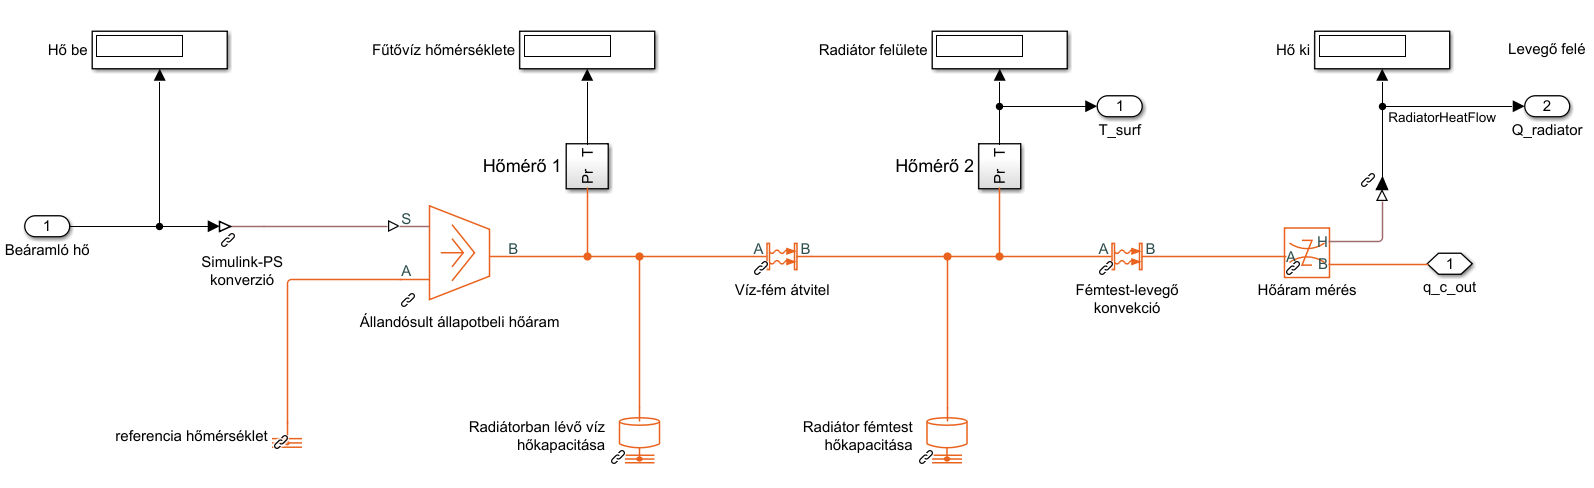
\includegraphics[trim=0 0 0 0, clip,width=\textwidth]{figures/simscape/radiator}
	\caption{Radiátor Simscape modellje}
	\label{fig:SimscapeRadiator}
\end{figure}

A felmelegedéskor és lehűléskor a pontos hőleadást akkor tudjuk modellezni, ha ismerjük a radiátor hőkapacitását. Ehhez tudnunk kell, hogy a radiátorban mennyi víz van, illetve hogy a radiátortest milyen nehéz.
A radiátorokat mindig az adott helyiséghez méretezik, ezért az adatokat leolvasással vagy katalógusból kapjuk normál esetben. A modellezéshez választanom kellett egy típust. Itt még csak paraméteresen kellene megadni az értékeket, vagy előbb a ház modelljét, hőszükségletét felírni, hiszen a házhoz tervezzük a fűtést és nem fordítva.

Radiátor katalógusokból\footnote{Purmo Ventil Compact - purmo.com/hu/termekek/lapradiatorok/purmo-ventil-compact.htm} azt találtam, hogy az egyes radiátor típusokra ezek a paraméterek milyen értékűek.

A termikus modell paraméterei egy 90 cm magas, 1,8 m hosszú C22 típusú radiátorra:

\begin{table}[H]
	\footnotesize
	\centering
	\caption{Radiátor adatai a tranziensekhez}
	%\renewcommand{\arraystretch}{2} % to increase cell height
	%\taburulecolor{gray}
	%\begin{tabular}{|p{0.8cm}|p{1cm}|p{1cm}|p{1cm}|p{1cm}|p{1cm}|p{1cm}|p{1cm}|}
	%
	%\begin{tabulary}{\linewidth}{LLc}
	\begin{tabu}{@{}ll@{}}
		\hline
		fémtest tömege 	& 90 \si[per-mode=symbol]{\kilogram}
		\\
		fémtest fajhője	& 464 \si[per-mode=symbol]{\joule\per\kilogram\per\kelvin}
		\\
		fűtővíz tömege	& 16 \si[per-mode=symbol]{\kilogram}
		\\
		víz fajhője		& 4189 \si[per-mode=symbol]{\joule\per\kilogram\per\kelvin}
		\\ \hline
	\end{tabu}
	\label{tab:RadiatorHeatCap}
	%
	%\label{tab:TabularExample}
	%\tabref{TabularExample}~táblázat
\end{table}

% \begin{table}[H]
	\centering
	
	\renewcommand{\arraystretch}{2} % to increase cell height
	\taburulecolor{gray}
	
	%\begin{tabular}{|p{0.8cm}|p{1cm}|p{1cm}|p{1cm}|p{1cm}|p{1cm}|p{1cm}|p{1cm}|}
	
	\newcolumntype{C}[1]{>{\centering\arraybackslash}p{#1}}
	\newcolumntype{R}[1]{>{\raggedleft\arraybackslash}p{#1}}
	
	\begin{tabu}{|p{4cm}|p{3cm}|p{3cm}|p{3cm}|c|}
		\cline{2-5}
		\multicolumn{1}{l|}{} 	& Komponens & hőleadás módja & Hőtároló tömeg & Fajhő \\ \cline{2-5}
		\multicolumn{5}{c}{}\\ \hline
		% header
%		\multirow{2}{*}
%		{Radiátor} & \multicolumn{2}{c|}{Time} \\	\cline{2-3}
%		& First flight & Second flight\\ \hline
		
		
		\multirow{2}{*}
					{Radiátor} 	 & Víz 		&	&  	&	\\  \cline{2-5}
								 & Fémtest 	&	& 	& 	\\  \hline
								 
		\multicolumn{5}{c}{}\\ \hline
		
		\multirow{3}{*}
					{Padlófűtés} & Víz 		&	&  	&	\\  \cline{2-5}
								 & Födém 	&	&  	&	\\  \cline{2-5}
								 & Padló burkolat 	& 	&	& 	\\  \hline
	\end{tabu}						
		% entries - event names aligned left with multicolumn
%		\multicolumn{1}{|l|}{flightHAT turned on} 	& & \\ \hline
%%		{|p{3cm}|p{1cm}|p{3cm}|p{3cm}|p{3cm}|}
%		%{p{1.5cm}|C{0.8cm}|C{0.8cm}|C{0.8cm}|C{0.8cm}|C{0.8cm}|C{0.8cm}|C{0.8cm}|C{0.8cm}|}
%		%\multicolumn{1}{l}{}&\multicolumn{8}{l}{SDO header (első adatbyte) - master kérése}
%		%\\ 		\cline{2-9}\cline{2-9}
%		\hline
%		felület& méret & kalorikus hőátbocsátási tényező    & hőtároló tömeg & hőkapac
%		
%		\\ \hline
%		külső fal & 4.5 \si{\metre\squared} & 2 \si[per-mode=fraction]{\watt\per\metre\squared\per\kelvin} & 4.5*200kg & e.g. 4.5*200*840 \si[per-mode=fraction]{\joule\per\kelvin}
%		\\ \hline
%		ablak & 4 \si{\metre\squared} & 4 \si[per-mode=fraction]{\watt\per\metre\squared\per\kelvin} & 0 & 0
%		\\ \hline
%		belső válaszfalak & 50 \si{\metre\squared} & 7 & 50*100kg & 50*100*840	
%		\\ \hline
%		padló & 16 \si{\metre\squared} & 11 & 16*200kg & 169*200*840	
%		\\ \hline
%		mennyezet & 16 \si{\metre\squared} & ? rad / conv &  & 	
%%		\\ \hline

	
	\caption{Fűtőtestek termikus tulajdonságai}
	\label{table-sdotypes}
\end{table}
 helzett

A radiátor hossza, magassága, konstrukciója alapján a tömegek kiszámíthatók, illetve az acél hőkapacitása katalógusadatként szerepel.
A szimulációban a  Simscape termikus hőtároló elem blokkjaiba a fenti adatokat írtam.%, a víz fajhője még egy hőtároló elem.


\section{Padlófűtés modellje}

A padlófűtések felépítése az alábbi ábrán található. Egy hőszigetelő rétegre kerülnek a műanyag csövek, bizonyos elrendezésben. Erre híg betont öntenek, hogy az a csövek teljes felületét körbevegye, ne alakuljanak ki zárványok. Ha a beton nem veszi teljesen körbe a fűtéscsöveket, a padlófűtés teljesítménye lecsökken. A beton hőellenállása nem hanyagolható el, ezért a szimulációban ezt a hőmérsékletesést is figyelembe veszem.

\begin{figure}[H]
	\centering
	% trim={<left> <lower> <right> <upper>}
	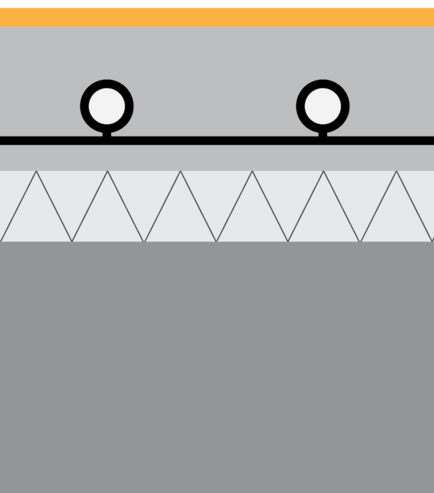
\includegraphics[trim=0 0 0 0, clip,width=0.25\textwidth]{figures/ISO11855typeA}
	\caption{Padlófűtés felépítése}
	\label{fig:futotest-padlofutes}
\end{figure}

\textit{Olesen} számításait használtam a méretezéshez.
A \SI{18}{\metre\squared} alapterületű helyiségben \SI{15}{\metre\squared}-nek vettem a fűtött területet. Ebből, és a hőigényből 45\si[per-mode=symbol]{\watt\per\metre\squared} teljesítményigény adódott.

Az előremenő vízhőmérséklet számítása:

Nyilvánvalóan nehéz lenne a felírt modellt egyénileg validálni, főleg hogy sehol sem találkoztam ilyen formában felírt képlettel a szakirodalomban. Szerencsére Cholewa \cite{CHOLEWA2013599} és Koca \cite{Koca} végzett méréseket falfűtés és mennyezetfűtés esetére. Ezen mérési eredmények paramétereit helyettesítettem be a hőleadás egyenletébe ahhoz hogy eldöntsem, helytálló-e a felírt modell. Az említett publikációkban minden adat rendelkezésre áll. A következő eseteket vizsgáltam:

\begin{table}[H]
	\vspace{12pt}
	\centering
	\renewcommand{\arraystretch}{1.4} % to increase cell height..
	\begin{tabular}{
			l
			S[table-format=-3.2]
			S[table-format=-3.2]
			S[table-format=-3.2]
			S[table-format=-3.2]
			S[table-format=-3.2]
			%cccc
		}
		%\hline
		\multicolumn{1}{c}{Paraméter} & \multicolumn{5}{c}{Cholewa mérései}\\%& \multicolumn{1}{c}{dummy} \\
		\hline%\cline{1-2}
		%	$T_{water}$    & Description & Price & (\$) \\
		%	\hline
		$T_{water},\si{\celsius}$      								& 30	& 30	& 40	& 50	& 55   		\\
		%$\dot{m}$ [\si[per-mode=fraction]{\kilogram\per\second}]  	& 0.0167& 0.055	& 0.0167& 0.0167& 0.055    	\\
		$\dot{m}$ [\si[per-mode=fraction]{\kilogram\per\minute}]  	& 1		& 3		& 1		& 1		& 3		    \\
		$T_{surf}$													& 25.3	& 26.2	& 32    & 37.4  & 42.4		\\
		$T_{a0.6}$       											& 22.3  & 23.3 	& 26.9	& 30.8  & 34.3 		\\
		$h_{total0.6}$ \small{$\left[ \frac{\si{\watt}}{\si{\metre\squared\kelvin}} \right]$ }
		& 8.7   & 9.4  	& 9.7  	& 10.5  & 10.8  	\\[5pt] \hline 
		%$\Delta T$       											& 3     & 2.9	& 5.1  	& 6.6   & 8.1 		\\[5pt] \hline 
		$q_{total}$ \small{$\left[ \frac{\si{\watt}}{\si{\metre\squared}} \right]$}
		& 25.1  & 26.4  & 47.8  &  68.8	& 88.4   	\\[5pt] 		
		$q_{formula}$ \small{$\left[ \frac{\si{\watt}}{\si{\metre\squared}} \right]$}
		& 24.6  & 26.7  & 46.3  &  64.5 & 85.5   	\\[5pt] %\hline 
		Pontosság [\%]
		& 98	& 101	&  97	& 93.75 & 96.7		\\ %\hline
		\hline
	\end{tabular}
	\caption{A \ref{eq_holeadas4}. képlettel kapott eredmények és a \cite{CHOLEWA2013599} és \cite{Koca} eredményeinek összevetése}
	
\end{table}


% Az 1.1 méréseket használva rendre 10%-kal alábecsültük a hőt.
{\Large }


A hőleadás egyenletével számolt és a fent hivatkozott, méréssel kapott eredmények elég jól követik egymást. Padlófűtésnél a padló felületi hőmérséklettel számoltam, ugyanis a padló hőmérséklete jóval alacsonyabb, mint a fűtővíz hőmérséklete.
A fenti publikációkban figyelembe vették a hőleadási tényező hőmérsékletfüggését.\footnote{Intuitívan is belátható, hogy melegebb testnek nagyobb a konvektív hőleadási tényezője. A konvektív hőátadás mértéke nagyban függ attól, hogy a felületen milyen sebességgel áramlik a levegő, hiszen a forró tea gyorsabban hűl, ha fújjuk, illetve szélben a kinti hőmérséklet kisebbnek érződik. Hasonlóan melegebb tárgy esetén a légáramlás felgyorsul, amiatt hogy a melegebb levegő felfelé száll.} %Nagyobb felületi légáramlás tehát megnövekedett konvektív hőátadást eredményez.}
Azaz a felfutási tranziens során is változik a hőátadási tényező.



\pagebreak